\documentclass[11pt,a4paper]{article}

\usepackage[T1]{fontenc}
\usepackage{lmodern}
\usepackage[english]{babel}
\usepackage[margin=1.15in]{geometry}
\usepackage{amsmath,amssymb,amsthm,mathtools}
\usepackage{microtype}
\usepackage{booktabs}
\usepackage{enumitem}
\usepackage{tikz}
\usepackage{pgfplots}
\usepackage[hidelinks]{hyperref}

\pgfplotsset{compat=1.18}
\usetikzlibrary{arrows.meta}

\hypersetup{
  pdftitle={On Feline Complexity},
  pdfauthor={Steve Andy Ildefonso Santos},
  pdfsubject={Control, persuasion and free boundaries in Felis catus}
}

\pgfplotsset{
  revista/.style={
    width=0.74\linewidth,
    height=5.2cm,
    axis lines=left,
    axis line style={-, gray!70},
    tick style={gray!70},
    tick label style={font=\footnotesize},
    label style={font=\small},
    every axis plot/.append style={line width=0.9pt},
    clip=false
  }
}

\newcommand{\gatoqed}{%
  \tikz[baseline=-0.1ex, x=0.95ex, y=0.95ex]{
    \fill (-0.82,0.25) -- (-0.82,1.2) -- (-0.15,0.72) -- cycle;
    \fill (0.82,0.25) -- (0.82,1.2) -- (0.15,0.72) -- cycle;
    \fill (0,0.1) ellipse (0.92 and 0.78);
    \fill[white] (-0.36,0.22) circle (0.15);
    \fill[white] (0.36,0.22) circle (0.15);
  }%
}
\renewcommand{\qedsymbol}{\gatoqed}

\theoremstyle{plain}
\newtheorem{teorema}{Theorem}[section]
\newtheorem{proposicion}[teorema]{Proposition}
\newtheorem{corolario}[teorema]{Corollary}
\newtheorem{conjetura}[teorema]{Conjecture}
\theoremstyle{definition}
\newtheorem{definicion}[teorema]{Definition}
\newtheorem{problema}[teorema]{Open Problem}
\theoremstyle{remark}
\newtheorem{observacion}[teorema]{Remark}

\numberwithin{equation}{section}

\DeclareMathOperator{\hol}{hol}
\newcommand{\R}{\mathbb{R}}
\newcommand{\E}{\mathbb{E}}
\renewcommand{\P}{\mathbb{P}}
\newcommand{\cg}{C}
\newcommand{\calib}{{\ensuremath{^{\ddagger}}}}
\newcommand{\costo}{\operatorname{cost}}
\newcommand{\OPT}{\operatorname{OPT}}
\newcommand{\prob}[1]{\textnormal{\textsc{#1}}}

\begin{document}

\begin{center}
  {\LARGE\bfseries On Feline Complexity:\par}
  \vspace{0.35em}
  {\Large Holonomy, Bayesian Persuasion, Free-Boundary Problems,\par
  and a General Theory of Minimal Effort in \textit{Felis catus}\par}
  \vspace{1.3em}
  {\large Steve Andy Ildefonso Santos\par}
  \vspace{0.4em}
  {\small Independent Laboratory of Applied Felinometry\par
  \texttt{github.com/stiffis}\par}
  \vspace{0.8em}
  November 5, 2026
\end{center}

\begin{abstract}
\noindent
The domestic cat is commonly described as lazy. I show that this is a modeling error: the cat solves, with provable bounds, several optimization problems that its caretakers have not even noticed they are losing.
(i)~I define the \emph{feline complexity} of a task as the minimal energy of a program executed on a human, prove an invariance theorem up to a training constant, and deduce that almost no craving is compressible, which explains the staring.
(ii)~Mid-air righting is a holonomy: the net rotation is the area enclosed in shape space. A cat with constant inertia cannot turn, and the isoperimetric inequality yields a minimum height $h_{\min}=2\pi^2 g/(\varepsilon v^2)$.
(iii)~The meow is an optimal Bayesian experiment: a cat that also meows when full, with probability $q^\star$, gets fed with probability $\mu_0/\mu^\star$ without ever lying in the technical sense. Across $n$ households that do not communicate, the yield is linear in $n$; a whiteboard on the fridge bounds it by $1$.
(iv)~Asking for the door and not walking through it is the rational holding of a real option with threshold $x^\star=\beta I/(\beta-1)$. The human bears the waiting cost, the expected time the door stays open can be infinite, and under a natural calibration the cat stays on the threshold forever with probability exactly $1/\varphi$.
(v)~Relocating after a sun patch satisfies the marginal value theorem, with optimal interval $T^\star=(3cW^2/2Rv^2)^{1/3}$.
(vi)~Algorithmically, the cat is an adversary: if it goes quiet when you get up at 3\,a.m., no policy gets below competitive ratio $2-1/B$, not even with randomness; if it hides in the last place on your list, the cost per search is maximal; and while placing one cat is linear, placing a colony is NP-complete.
I conclude that the cat does not avoid work. It outsources it.
\end{abstract}

\section{Introduction}

Many species that have been studied prefer to work for their food even when free food sits right beside it, a phenomenon known as \emph{contrafreeloading}. Delgado, Han and Bain~\cite{delgado} offered 17 domestic cats a food puzzle and a tray of food. The cats mostly chose the tray. The literature received this as an anomaly; here I take it as an axiom.

\medskip
\noindent\textbf{Axiom 0.} \emph{The cat minimizes its own effort subject to getting what it wants, and regards the human as part of the environment.}

\medskip
The indirect evidence is abundant. Cats can tell their name from other words~\cite{saito}, so failing to come when called cannot be attributed to a recognition problem. They embed in the purr a high-pitched component that humans perceive as more urgent~\cite{mccomb}. They flow until they fill their container~\cite{fardin}, recover from stress sooner when given a box~\cite{vinke}, and will even sit in squares that exist only as illusory contours~\cite{smith}. Their way of drinking balances inertia and gravity to within order one~\cite{reis}.

My contribution is to bring these behaviors under a single principle and to state results that can actually be proved. \S\ref{sec:complejidad} formalizes feline complexity. The following sections treat the fall (\S\ref{sec:caida}), the meow (\S\ref{sec:maullido}), the door (\S\ref{sec:puerta}) and the sun (\S\ref{sec:sol}). \S\ref{sec:computacional} analyzes the cat as an algorithmic adversary. \S\ref{sec:menores} collects minor results, including why the cat sits on your keyboard, and \S\ref{sec:abiertos} lists open problems.

\medskip
\noindent\textbf{Honesty note.} The proofs are correct within their models. The models are caricatures. Every parameter marked \calib\ I calibrated by eye rather than measured, and it is there only to produce numbers. The empirical claims attributed to the literature are real and cited. The computations can be reproduced with \texttt{revision\_por\_patas.py}, the program that accompanies this work and serves as its peer review; Spanish for ``review by paws.'' The symbol closing each proof is a cat, for reasons that require no justification.

\section{Feline complexity}\label{sec:complejidad}

\begin{definicion}[Cat--human system]\label{def:sistema}
Let $\Sigma$ be a finite alphabet of $k\ge 2$ \emph{acts} (meowing, rubbing, staring, moving a paw toward a glass) with energy cost $e:\Sigma\to(0,\infty)$, and let $\mathcal T$ be a set of \emph{tasks}. A \emph{human} is a partial function $H:\Sigma^*\to\mathcal T$. The energy of a program $p=a_1\cdots a_m$ is $E(p)=\sum_i e(a_i)$.
\end{definicion}

\begin{definicion}[Feline complexity]
The feline complexity of $T\in\mathcal T$ relative to $H$ is
\begin{equation}
  \cg_H(T)=\inf\{\,E(p) : H(p)=T\,\},
\end{equation}
with $\inf\varnothing=\infty$. I say that $H$ is \emph{trainable to} $H'$ if there exists $t\in\Sigma^*$ such that $H(tp)=H'(p)$ for all $p\in\Sigma^*$. The word $t$ is called a \emph{training protocol}.
\end{definicion}

The analogy with Kolmogorov complexity~\cite{kolmogorov,livitanyi} is deliberate: the cat writes the programs and the human runs them.

\begin{teorema}[Invariance]\label{teo:invariancia}
If $H$ is trainable to $H'$ via $t$, then for every task $T$,
\begin{equation}
  \cg_H(T)\le \cg_{H'}(T)+E(t).
\end{equation}
If moreover $H'$ is trainable to $H$ via $t'$, then $|\cg_H(T)-\cg_{H'}(T)|\le\max\{E(t),E(t')\}$ whenever both complexities are finite.
\end{teorema}

\begin{proof}
If $H'(p)=T$, then $H(tp)=T$ and $E(tp)=E(t)+E(p)$. I take the infimum over $p$. The second part follows by symmetry.
\end{proof}

Feline complexity is thus a property of the task and not of your family, up to a constant that depends only on how fast the household gives in.

\begin{observacion}[Amortization]
A real human has memory: $t$ is paid once. Over $m$ tasks, the training cost per task is $E(t)/m\to 0$. This is a capital investment, and it explains why the cat's first week at home seems so much louder than the ones that follow.
\end{observacion}

\begin{teorema}[Incompressibility of cravings]\label{teo:incompresible}
Suppose $e\equiv 1$ and $|\mathcal T|=k^n$. For every human $H$ and every integer $0\le c<n$, the fraction of tasks with $\cg_H(T)<n-c$ is at most
\begin{equation}
  \frac{k^{n-c}-1}{(k-1)\,k^{n}}<\frac{k^{-c}}{k-1}.
\end{equation}
\end{teorema}

\begin{proof}
There are $\sum_{i<n-c}k^i=(k^{n-c}-1)/(k-1)$ words of length less than $n-c$, and each produces at most one task.
\end{proof}

With $k=4$, $n=10$ and $c=2$, $97.9\%$ of cravings require at least eight acts. The average human reads this bound as ``I don't know what it wants.'' The cat reads it as a reason to keep staring.

\begin{corolario}[Telepathy]
At most one task has complexity zero: the one $H$ performs on the empty word, without anyone asking for anything. Every cat works to make that task breakfast.
\end{corolario}

\begin{teorema}[Meow code, Shannon~\cite{shannon}]\label{teo:codigo}
If cravings follow a distribution $\pi$ and the cat uses a uniquely decodable code over $k$ acts, its expected number of acts per craving is at least the entropy $\mathcal H_k(\pi)=-\sum_T\pi(T)\log_k\pi(T)$.
\end{teorema}

Table~\ref{tab:codigo} shows the dyadic case, where the bound is attained. A cat with two phonemes (short meow and long meow) and those frequencies cannot do better than $1.75$ acts per craving. I note that the optimal code assigns tuna the shortest word, in full agreement with what is observed in any kitchen when a can is opened.

\begin{table}[ht]
\centering
\caption{Huffman code for a repertoire with calibrated frequencies\calib.}\label{tab:codigo}
\begin{tabular}{lccc}
\toprule
Craving & $\pi(T)$ & Word & Acts \\
\midrule
Tuna & $1/2$ & \texttt{0} & 1 \\
Door & $1/4$ & \texttt{10} & 2 \\
Lap & $1/8$ & \texttt{110} & 3 \\
That you stop what you are doing & $1/8$ & \texttt{111} & 3 \\
\midrule
\multicolumn{2}{l}{Expected length $=\mathcal H_2(\pi)$} & & $1.75$ \\
\bottomrule
\end{tabular}
\end{table}

\begin{proposicion}[Inscrutability]\label{prop:noComputable}
If tasks are binary strings, $e\equiv 1$ and $H$ is a universal machine, then $\cg_H$ is Kolmogorov complexity and is consequently not computable~\cite{livitanyi}.
\end{proposicion}

In other words: if your human is universal, no algorithm computes how hard it is for your cat to ask you for something. The question ``what does it want now?'' was never rhetorical. In its quantitative version, it is uncomputable.

\section{The fall as a holonomy}\label{sec:caida}

In 1894, Marey~\cite{marey,marey-nature} photographed a cat falling with no initial rotation and landing on its feet, which seemed to contradict the conservation of angular momentum. Kane and Scher~\cite{kanescher} gave the dynamical explanation and Montgomery~\cite{montgomery} reformulated it as a holonomy in gauge theory. Here I study a poorer abelian model that admits closed-form bounds.

\begin{definicion}[Coaxial cat]
Two coaxial bodies, front and rear, with angles $\theta_1,\theta_2$ and inertias $I_1(t),I_2(t)>0$ that the cat controls by tucking or extending its legs. It starts at rest, so $I_1\dot\theta_1+I_2\dot\theta_2=0$ throughout the fall. Its \emph{shape} is $(\psi,\lambda)$, with twist $\psi=\theta_1-\theta_2$ and inertia share $\lambda=I_2/(I_1+I_2)\in(0,1)$.
\end{definicion}

\begin{teorema}[Rotation is an area]\label{teo:holonomia}
In the coaxial cat, $\dot\theta_1=\lambda\dot\psi$ and $\dot\theta_2=(\lambda-1)\dot\psi$. Hence, for every closed loop $\gamma$ in shape space, both bodies rotate by the same amount:
\begin{equation}
  \Delta\theta=\hol(\gamma)=\oint_\gamma\lambda\,d\psi=\iint_{D}d\lambda\wedge d\psi .
\end{equation}
For a simple loop, $|\Delta\theta|$ is the enclosed area, and the rotation is positive when $\gamma$ runs clockwise in the $(\psi,\lambda)$ plane.
\end{teorema}

\begin{proof}
The formulas give $I_1\lambda\dot\psi+I_2(\lambda-1)\dot\psi=\dot\psi\,(I_1I_2-I_2I_1)/(I_1+I_2)=0$, and they are consistent with $\dot\theta_1-\dot\theta_2=\dot\psi$. Integrating, $\Delta\theta_1=\oint\lambda\,d\psi$ and $\Delta\theta_2=\oint\lambda\,d\psi-\oint d\psi=\Delta\theta_1$. The rest is Stokes' theorem.
\end{proof}

The net rotation does not depend on how fast the loop is traversed, only on its geometry: the cat is not ``pushing'' against anything. The $1$-form $\lambda\,d\psi$ is the connection and $d\lambda\wedge d\psi$ its curvature.

\begin{corolario}[A rigid cat crashes]\label{cor:rigido}
If $\lambda$ is constant, $\hol(\gamma)=\lambda\oint d\psi=0$. With constant inertia, no sequence of twists produces net rotation. Tucking the legs is not decoration: it is what gives shape space its second dimension.
\end{corolario}

\begin{corolario}[Minimum twist]\label{cor:torsion}
Let $k>1$ be the ratio of extended to tucked inertia, so that $\lambda$ ranges over an interval of length at most $\Delta\lambda=(k-1)/(k+1)$. A simple loop producing a turn of $\pi$ requires a twist of amplitude
\begin{equation}
  \Psi\ge\frac{\pi}{\Delta\lambda}=\pi\,\frac{k+1}{k-1}>\pi.
\end{equation}
No inertia ratio, however favorable, lets a coaxial cat turn over in a single cycle with less than $180^\circ$ of twist.
\end{corolario}

\begin{proof}
A simple loop inside the rectangle $\Psi\times\Delta\lambda$ encloses area at most $\Psi\,\Delta\lambda$, and this must be at least $\pi$.
\end{proof}

To fix the cost of the loop, I equip shape space with the metric $ds^2=d\psi^2+\varepsilon^{-2}d\lambda^2$, where $\varepsilon>0$ measures how much more it costs to move the legs than to twist the spine, and I bound the shape speed by $|\dot c|\le v$.

\begin{teorema}[Isoholonomy]\label{teo:isoholonomia}
Every loop $\gamma$ with $|\hol(\gamma)|=\Delta$ has length $L$ satisfying $L^2\ge 4\pi\Delta/\varepsilon$, and its energy over a time $T$ satisfies
\begin{equation}
  \int_0^T|\dot c|^2\,dt\ge\frac{4\pi\Delta}{\varepsilon T}.
\end{equation}
Equality holds only for a metric circle traversed at constant speed, that is, an ellipse in the coordinates $(\psi,\lambda)$.
\end{teorema}

\begin{proof}
With $y=\lambda/\varepsilon$ the metric is Euclidean and $\Delta=\varepsilon\,|\oint y\,d\psi|$. For closed curves, not necessarily simple, with winding number $w$, the Banchoff--Pohl inequality~\cite{banchoffpohl} gives $L^2\ge 4\pi\iint w^2\ge 4\pi\left|\iint w\right|=4\pi\Delta/\varepsilon$, since $w$ is an integer. The energy bound is Cauchy--Schwarz: $L^2\le T\int|\dot c|^2\,dt$. Equality requires $\gamma$ to be a circle and $|\dot c|$ to be constant.
\end{proof}

\begin{corolario}[Minimum height]\label{cor:altura}
With $T=\sqrt{2h/g}$, a cat that makes $n$ circular laps to turn by $\pi$ needs
\begin{equation}
  h_{\min}(n)=n\,\frac{2\pi^2 g}{\varepsilon v^2}.
\end{equation}
A metric square of the same area spends a factor $4/\pi$ of energy, that is, $27.3\%$ more than the circle. Rounding the corners pays off.
\end{corolario}

\begin{proof}
With $n$ laps around a disk of area $\pi/(n\varepsilon)$, $L=2\pi\sqrt{n/\varepsilon}$. The bound $L\le vT$ gives the result. For the square, $L_\square^2/L_\circ^2=16\,(\pi/\varepsilon)/(4\pi^2/\varepsilon)=4/\pi$.
\end{proof}

\begin{figure}[ht]
\centering
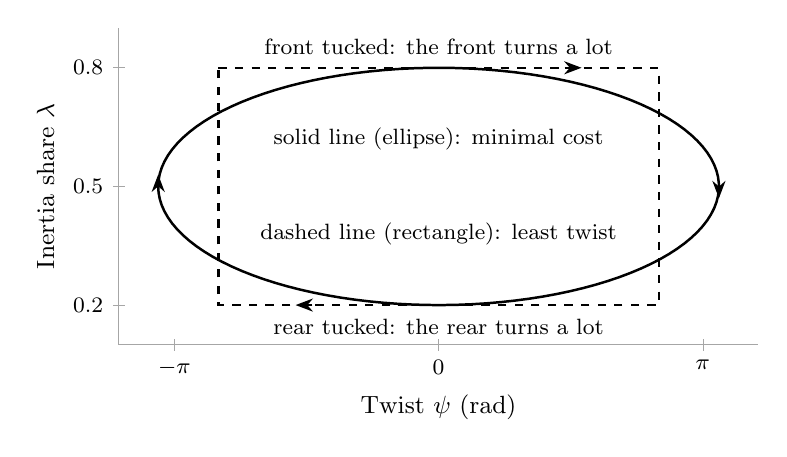
\begin{tikzpicture}
\begin{axis}[
  revista,
  width=0.8\linewidth,
  height=5.6cm,
  xlabel={Twist $\psi$ (rad)},
  ylabel={Inertia share $\lambda$},
  xmin=-3.8, xmax=3.8,
  ymin=0.1, ymax=0.9,
  xtick={-3.14159,0,3.14159},
  xticklabels={$-\pi$,$0$,$\pi$},
  ytick={0.2,0.5,0.8}
]
\addplot[black, dashed] coordinates {(-2.618,0.8) (2.618,0.8) (2.618,0.2) (-2.618,0.2) (-2.618,0.8)};
\addplot[black, domain=0:360, samples=120] ({-3.3333*cos(x)},{0.5+0.3*sin(x)});
\draw[-{Stealth[length=2.2mm]}, line width=0.9pt] (axis cs:1.5,0.8) -- (axis cs:1.7,0.8);
\draw[-{Stealth[length=2.2mm]}, line width=0.9pt] (axis cs:-1.5,0.2) -- (axis cs:-1.7,0.2);
\draw[-{Stealth[length=2.2mm]}, line width=0.9pt] (axis cs:3.3333,0.51) -- (axis cs:3.3333,0.47);
\draw[-{Stealth[length=2.2mm]}, line width=0.9pt] (axis cs:-3.3333,0.49) -- (axis cs:-3.3333,0.53);
\node[font=\footnotesize, anchor=south] at (axis cs:0,0.81) {front tucked: the front turns a lot};
\node[font=\footnotesize, anchor=north] at (axis cs:0,0.19) {rear tucked: the rear turns a lot};
\node[font=\footnotesize, fill=white, inner sep=1.5pt] at (axis cs:0,0.62) {solid line (ellipse): minimal cost};
\node[font=\footnotesize, fill=white, inner sep=1.5pt] at (axis cs:0,0.38) {dashed line (rectangle): least twist};
\end{axis}
\end{tikzpicture}
\caption{Two loops in shape space with $k=4$\calib, both of area $\pi$. By Theorem~\ref{teo:holonomia}, both flip the cat by exactly $180^\circ$.}\label{fig:formas}
\end{figure}

\begin{observacion}[The model refutes itself, and that is the interesting part]
I take $k=4$\calib, so $\Delta\lambda=0.6$ (Figure~\ref{fig:formas}). The rectangle demands $\Psi=300^\circ$ of twist; the ellipse, $382^\circ$.\footnote{The half-width of the rectangle is $\pi/1.2=2.61799\ldots$, which agrees with $\varphi^2=2.61803\ldots$ to four decimal places. It means nothing, but I could not help noticing, and $\varphi$ will reappear in \S\ref{sec:puerta} for legitimate reasons.} With a more reasonable twist of $90^\circ$\calib\ it would take $n=5$ laps, which in a fall of $30$\,cm ($T=0.247$\,s) means about $20$\,Hz. Nobody has reported a cat falling at $20$\,Hz. I conclude that tuck-and-turn is not enough and that the real cat must bend: this is the Kane--Scher way out, whose model bends without twisting and whose holonomy is non-abelian~\cite{kanescher,montgomery}. My model does not describe the cat. It shows, instead, why the cat has to be smarter than my model.
\end{observacion}

\section{The meow as a Bayesian experiment}\label{sec:maullido}

\begin{definicion}[Dinner game]
The state of the cat is $\omega\in\{\text{hungry},\text{full}\}$, with $\P(\text{hungry})=\mu_0$. The human gains $b>0$ from feeding a hungry cat and loses $a>0$ from feeding a full one, so they serve food if and only if their belief satisfies $\mu\ge\mu^\star=a/(a+b)$. The cat only wants to eat, in every state. Before the day begins, it chooses a meowing policy $\pi(\text{meow}\mid\omega)$, which the human knows from accumulated experience.
\end{definicion}

\begin{teorema}[Optimal meow, Kamenica--Gentzkow~\cite{kamenica}]\label{teo:maullido}
If $\mu_0<\mu^\star$, the maximal probability of being fed is $\mu_0/\mu^\star$, attained by
\begin{equation}
  \pi(\text{meow}\mid\text{hungry})=1,
  \qquad
  \pi(\text{meow}\mid\text{full})=q^\star=\frac{\mu_0\,(1-\mu^\star)}{(1-\mu_0)\,\mu^\star}.
\end{equation}
\end{teorema}

\begin{proof}
\emph{Bound.} Every policy induces a random posterior belief $\mu$ with $\E[\mu]=\mu_0$. By Markov's inequality, $\P(\mu\ge\mu^\star)\le\mu_0/\mu^\star$. \emph{Attainment.} Under the stated policy, $\P(\text{meow})=\mu_0+(1-\mu_0)q^\star=\mu_0/\mu^\star$, and Bayes' rule gives $\mu_0/(\mu_0/\mu^\star)=\mu^\star$ as the belief after a meow. Silence reveals fullness with certainty and the human does not serve; the meow leaves the human exactly indifferent, and they serve.
\end{proof}

\begin{figure}[ht]
\centering
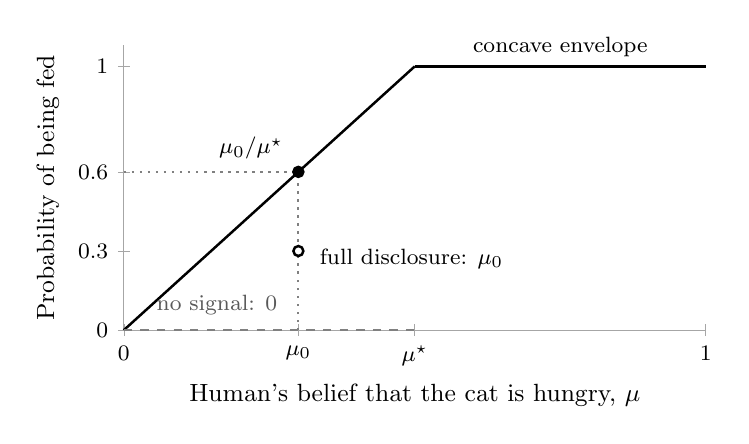
\begin{tikzpicture}
\begin{axis}[
  revista,
  xlabel={Human's belief that the cat is hungry, $\mu$},
  ylabel={Probability of being fed},
  xmin=0, xmax=1,
  ymin=0, ymax=1.08,
  xtick={0,0.3,0.5,1},
  xticklabels={$0$,$\mu_0$,$\mu^\star$,$1$},
  ytick={0,0.3,0.6,1}
]
\addplot[black, domain=0:0.5, samples=2] {2*x};
\addplot[black, domain=0.5:1, samples=2] {1};
\addplot[gray, dashed] coordinates {(0,0) (0.4985,0)};
\addplot[gray, dotted, thick] coordinates {(0.3,0) (0.3,0.6)};
\addplot[gray, dotted, thick] coordinates {(0,0.6) (0.3,0.6)};
\addplot[only marks, mark=*, mark size=1.8pt, black] coordinates {(0.3,0.6)};
\addplot[only marks, mark=*, mark size=1.8pt, black, mark options={fill=white}] coordinates {(0.3,0.3)};
\node[font=\footnotesize, anchor=south east] at (axis cs:0.29,0.61) {$\mu_0/\mu^\star$};
\node[font=\footnotesize, anchor=west] at (axis cs:0.32,0.27) {full disclosure: $\mu_0$};
\node[font=\footnotesize, anchor=south] at (axis cs:0.75,1.0) {concave envelope};
\node[font=\footnotesize, anchor=south, text=gray!70!black] at (axis cs:0.16,0.02) {no signal: $0$};
\end{axis}
\end{tikzpicture}
\caption{Concavification with $\mu_0=0.3$ and $\mu^\star=0.5$\calib. Meowing strategically doubles the probability of dinner relative to always telling the truth.}\label{fig:concavo}
\end{figure}

With $\mu_0=0.3$ and $\mu^\star=0.5$\calib\ (Figure~\ref{fig:concavo}), I get $q^\star=3/7$: the full cat meows $43\%$ of the time and eats with probability $0.6$. If it were always transparent it would eat with probability $0.3$, and if it never conveyed anything it would never eat at all. This is not a lie in the technical sense: the human knows the policy, updates correctly, and serves anyway. The high-pitched component of the purr documented by McComb et al.~\cite{mccomb} suggests that the cat also moves $\mu^\star$ from the human's side.

\begin{proposicion}[Six dinners]\label{prop:seis}
Let $n$ households play the dinner game independently, without observing one another, and let $p=\min\{1,\mu_0/\mu^\star\}$. The number of dinners $D_n$ is binomial and $\E[D_n]=np$. If the households share a log of dinners served, and therefore stop serving after the first, the expected value falls to $1-(1-p)^n\le 1$. The waste avoided, $np-1+(1-p)^n$, is nonnegative and asymptotically linear in $n$.
\end{proposicion}

\begin{proof}
Independence gives the binomial. With a log, the cat eats if and only if at least one household would have served. Nonnegativity is Bernoulli's inequality.
\end{proof}

With $n=6$ and $p=0.6$, this goes from $3.6$ dinners to $0.9959$. If $\mu_0\ge\mu^\star$, then $p=1$ and $D_6=6$ with certainty, a regime documented in the children's literature~\cite{moore}. The corrective mechanism is a whiteboard on the fridge. Its deployment faces the practical problem that whoever uses it has already served dinner.

\section{The door as a real option}\label{sec:puerta}

The cat asks for the door. You open it. It sits on the threshold and looks outside. This behavior is considered irrational only because the standard analysis omits the value of waiting~\cite{mcdonaldsiegel,dixitpindyck}.

\begin{definicion}[Door problem]
The value of being outside follows $dX_t=\mu X_t\,dt+\sigma X_t\,dW_t$ with $X_0=x_0>0$. Leaving costs $I>0$ (the warmth given up), is irreversible for the purposes of the model, and is discounted at rate $r>\mu$. The cat solves $V(x)=\sup_\tau\E_x[e^{-r\tau}(X_\tau-I)^+]$. Let $\beta>1$ be the root of $\tfrac12\sigma^2\beta(\beta-1)+\mu\beta-r=0$.
\end{definicion}

\begin{teorema}[The cat's threshold]\label{teo:umbral}
The optimal policy is to leave when $X_t$ first reaches $x^\star=\frac{\beta}{\beta-1}I$, and
\begin{equation}
  V(x)=\begin{cases}(x^\star-I)\,(x/x^\star)^{\beta}, & x<x^\star,\\ x-I, & x\ge x^\star.\end{cases}
\end{equation}
\end{teorema}

\begin{proof}
Let $\mathcal L=\tfrac12\sigma^2x^2\partial_x^2+\mu x\partial_x-r$. The solutions of $\mathcal LV=0$ bounded at $0$ are $Ax^\beta$. The free-boundary conditions $V(x^\star)=x^\star-I$ and $V'(x^\star)=1$ determine $A$ and $x^\star$. It remains to check the variational inequality. On $x<x^\star$, $V$ is convex with tangent $x-I$ at $x^\star$, so $V\ge x-I$. On $x>x^\star$, $\mathcal L(x-I)=(\mu-r)x+rI\le 0$ is equivalent to $x\ge rI/(r-\mu)$, and $x^\star$ meets this bound because $\mu\beta-r=-\tfrac12\sigma^2\beta(\beta-1)<0$. Itô's lemma concludes.
\end{proof}

\begin{proposicion}[Why it protests when it has no plan to leave]\label{prop:protesta}
$V(x)>0$ for all $x>0$. Closing the door destroys an asset of positive value even if $x\ll I$, that is, even if leaving is of no use to the cat at all.
\end{proposicion}

This resolves the classical paradox: the cat does not want to go out, it wants to be \emph{able} to go out. By closing the door you liquidate an option.

\begin{teorema}[Externality]\label{teo:externalidad}
If the human bears a flow cost $c<rI$ while holding the door, the threshold maximizing joint welfare is
\begin{equation}
  x_S^\star=\frac{\beta}{\beta-1}\Bigl(I-\frac{c}{r}\Bigr)=x^\star-\frac{\beta}{\beta-1}\,\frac{c}{r}.
\end{equation}
Since the cat does not internalize $c$, it leaves too late, and the gap is linear in $c$.
\end{teorema}

\begin{proof}
The social value solves $\mathcal LW=c$, with solution $W(x)=Ax^\beta-c/r$. The conditions $W(x_S^\star)=x_S^\star-I$ and $W'(x_S^\star)=1$ give $x_S^\star/\beta-c/r=x_S^\star-I$, and I solve for $x_S^\star$.
\end{proof}

\begin{teorema}[Door-open time]\label{teo:tiempo}
Let $\tau$ be the first time $X$ reaches $x^\star$, with $x_0<x^\star$, and let $\nu=\mu-\sigma^2/2$.
\begin{enumerate}[label=(\alph*),nosep]
\item If $\nu>0$, $\E[\tau]=\ln(x^\star/x_0)/\nu$.
\item If $\nu=0$, $\tau<\infty$ almost surely, but $\E[\tau]=\infty$.
\item If $\nu<0$, $\P(\tau<\infty)=(x_0/x^\star)^{\,1-2\mu/\sigma^2}<1$, so that $\E[\tau]=\infty$.
\end{enumerate}
In every case, $\E[e^{-r\tau}]=(x_0/x^\star)^\beta$.
\end{teorema}

\begin{proof}
$\ln X_t$ is a Brownian motion with drift $\nu$, and I apply the classical first-passage results. For (c), with $\theta=1-2\mu/\sigma^2$, the process $X_t^{\theta}$ is a martingale, since $\theta\nu+\tfrac12\theta^2\sigma^2=0$, and I apply optional sampling, using $X_t\to 0$ on $\{\tau=\infty\}$. The last identity is optional sampling for $e^{-rt}X_t^\beta$.
\end{proof}

\begin{corolario}[The golden cat]\label{cor:aureo}
Let $\mu=0$ and $\sigma^2=2r$\calib, so that the outdoors is a martingale whose volatility exactly offsets patience. Then $\beta^2-\beta-1=0$, that is, $\beta=\varphi=(1+\sqrt5)/2$, and $x^\star=\varphi^2I$. With $x_0=I$:
\begin{equation}
  \P(\text{it ever leaves})=\varphi^{-2}\approx 0.382,
  \qquad
  \P(\text{it never leaves})=\varphi^{-1}\approx 0.618,
\end{equation}
and the value of the option is $V(I)=\varphi^{\,1-2\varphi}I\approx 0.341\,I$.
\end{corolario}

\begin{proof}
The characteristic equation is $r\beta(\beta-1)-r=0$. Moreover, $\varphi/(\varphi-1)=\varphi^2$, $1-\varphi^{-2}=\varphi^{-1}$ and $\varphi^2-1=\varphi$. I substitute into Theorems~\ref{teo:umbral} and~\ref{teo:tiempo}.
\end{proof}

\begin{figure}[ht]
\centering
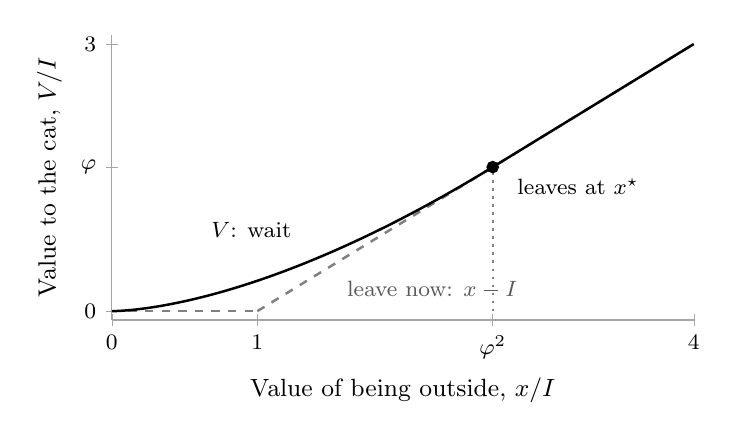
\begin{tikzpicture}
\begin{axis}[
  revista,
  xlabel={Value of being outside, $x/I$},
  ylabel={Value to the cat, $V/I$},
  xmin=0, xmax=4,
  ymin=-0.1, ymax=3.1,
  xtick={0,1,2.618,4},
  xticklabels={$0$,$1$,$\varphi^2$,$4$},
  ytick={0,1.618,3},
  yticklabels={$0$,$\varphi$,$3$}
]
\addplot[gray, dashed] coordinates {(1,0) (4,3)};
\addplot[gray, dashed] coordinates {(0,0) (1,0)};
\addplot[black, domain=0:2.618, samples=80] {0.340949*x^1.618034};
\addplot[black] coordinates {(2.618,1.618) (4,3)};
\addplot[gray, dotted, thick] coordinates {(2.618,0) (2.618,1.618)};
\addplot[only marks, mark=*, mark size=1.8pt, black] coordinates {(2.618,1.618)};
\node[font=\footnotesize, anchor=west] at (axis cs:2.72,1.4) {leaves at $x^\star$};
\node[font=\footnotesize, anchor=north west, text=gray!70!black] at (axis cs:1.55,0.45) {leave now: $x-I$};
\node[font=\footnotesize, anchor=south east] at (axis cs:1.3,0.72) {$V$: wait};
\end{axis}
\end{tikzpicture}
\caption{Value of the option under the golden calibration. $V$ always exceeds the immediate payoff and touches it tangentially at $x^\star$ (smooth pasting). The vertical distance between the two curves is what the cat is defending when you close the door.}\label{fig:puerta}
\end{figure}

I simulated $20{,}000$ cats with a Brownian bridge correction and got an exit fraction of $0.3820$, against $\varphi^{-2}=0.38197$. Taking the minute as the unit, $r=0.02$\calib, $\sigma^2=0.04$\calib\ and $c/r=I/4$\calib, I obtain $x^\star=2.618\,I$ and $x_S^\star=1.964\,I$ (Figure~\ref{fig:puerta}). The human pays, in present value, $(c/r)(1-\varphi^{-2\varphi})\approx 0.789\,c/r$ for a service that $61.8\%$ of the time ends without the cat leaving. In undiscounted time the expected cost is infinite, a result that anyone who has stood holding a door in winter will confirm.

\section{The sun patch}\label{sec:sol}

The sun moves. So does the cat, but only when it pays.

\begin{definicion}[Sun patch]
A patch of width $W$ moves at speed $v$. A cat at distance $\delta$ from its center receives power $P(\delta)=R(1-(2\delta/W)^2)$. Moving costs $c$ (which mainly consists of waking up). A cycle lasts $T$ with $vT\le W$, and the cat chooses where to resettle each cycle.
\end{definicion}

\begin{teorema}[Optimal interval and marginal value]\label{teo:sol}
It is optimal to resettle ahead of the patch's center, so that $\delta$ traverses the symmetric interval $[-vT/2,\,vT/2]$. The net rate is
\begin{equation}
  g(T)=R\Bigl(1-\frac{v^2T^2}{3W^2}\Bigr)-\frac{c}{T},
\end{equation}
strictly concave, with a unique maximum at
\begin{equation}
  T^\star=\Bigl(\frac{3cW^2}{2Rv^2}\Bigr)^{1/3}.
\end{equation}
Moreover, $P(vT^\star/2)=g(T^\star)$: the cat gets up exactly when the instantaneous power falls to its average net rate. This is Charnov's marginal value theorem~\cite{charnov}.
\end{teorema}

\begin{proof}
For fixed $T$, the mean of $P$ over an interval of length $vT$ is maximized by centering it, because $P$ is concave and symmetric. The integral gives $g$. Concavity on $T>0$ is immediate, and $g'(T)=0$ gives $T^\star$. At the optimum $c/T^\star=2R(vT^\star)^2/(3W^2)$. Substituting, $g(T^\star)=R(1-(vT^\star/W)^2)=P(vT^\star/2)$.
\end{proof}

\begin{figure}[ht]
\centering
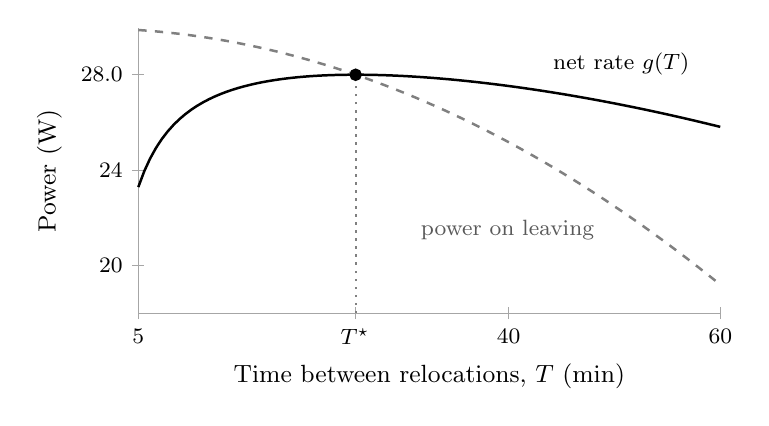
\begin{tikzpicture}
\begin{axis}[
  revista,
  xlabel={Time between relocations, $T$ (min)},
  ylabel={Power (W)},
  xmin=5, xmax=60,
  ymin=18, ymax=30,
  xtick={5,25.5,40,60},
  xticklabels={$5$,$T^\star$,$40$,$60$},
  ytick={20,24,28.04},
  yticklabels={$20$,$24$,$28.0$}
]
\addplot[black, domain=5:60, samples=100] {30*(1-(0.01*x)^2/3)-33.3333/x};
\addplot[gray, dashed, domain=5:60, samples=60] {30*(1-(0.01*x)^2)};
\addplot[gray, dotted, thick] coordinates {(25.54,18) (25.54,28.04)};
\addplot[only marks, mark=*, mark size=1.8pt, black] coordinates {(25.54,28.04)};
\node[font=\footnotesize, anchor=south east] at (axis cs:58,27.6) {net rate $g(T)$};
\node[font=\footnotesize, anchor=east, text=gray!70!black] at (axis cs:49,21.5) {power on leaving};
\end{axis}
\end{tikzpicture}
\caption{With $v=10^{-4}$\,m/s, $W=60$\,cm, $R=30$\,W and $c=2$\,kJ\calib, the maximum of $g$ falls where the power on leaving crosses it. The marginal value theorem, executed at $25.5$ minutes.}\label{fig:sol}
\end{figure}

Numerically (Figure~\ref{fig:sol}), $T^\star\approx 25.5$ minutes, during which the patch advances $15$\,cm, and $g(T^\star)\approx 28.0$\,W. The exponent $1/3$ is the signature of inventory problems, so the cat manages its heat the way a warehouse manages its stock. The law $T^\star\propto (W/v)^{2/3}$ is a falsifiable prediction, and I invite anyone with a window, a cat and a free afternoon to test it.

\section{Computational complexity}\label{sec:computacional}

So far I have measured joules. Now I measure steps. A point of terminology: calling the cat \emph{lazy} was always correct, but in the sense of lazy evaluation: it computes nothing until someone demands the result. I study three classical conflicts, in increasing number of cats.

\subsection{3\,a.m.: the cat as an adaptive adversary}

\begin{definicion}[The 3\,a.m.\ problem]
Each meow endured costs the human $1$. Getting up costs an integer $B\ge 2$ and ends the episode. The human does not know how many meows remain. The deterministic policy $j\ge 1$ endures $j-1$ meows and gets up on the $j$-th. If the cat emits $t$ meows in total,
\begin{equation}
  \costo(j,t)=\begin{cases}t, & t<j,\\ j-1+B, & t\ge j,\end{cases}
  \qquad
  \OPT(t)=\min\{t,B\}.
\end{equation}
A policy is $\rho$-competitive if $\E[\costo]\le\rho\,\OPT(t)$ for all $t$. This is the \emph{ski rental} problem, with skiing replaced by sleep.
\end{definicion}

\begin{teorema}[It goes quiet when you get up]\label{teo:adaptativo}
The policy $j=B$ is $(2-1/B)$-competitive and no deterministic policy does better. Moreover, if the cat watches the human and goes quiet the moment they get up, randomness does not help either: every randomized policy satisfies $\E[\costo]\ge(2-1/B)\,\E[\OPT]$, with $\OPT$ evaluated on the night that actually occurred.
\end{teorema}

\begin{proof}
With $j=B$: if $t<B$, the cost is $t=\OPT(t)$; if $t\ge B$, the cost is $2B-1$ and $\OPT(t)=B$. For the lower bound, given $j$, I take $t=j$. If $j\le B$, the ratio is $1+(B-1)/j\ge 2-1/B$; if $j>B$, it is $(j-1+B)/B\ge 2$. For the second part, let $M\ge 2B$ and I have the cat meow until the human gets up or until $M$ meows are reached. If the human gets up on meow $j$, I apply the above with $t=j$. If not, they pay $M$ against $\OPT=B$, and $M/B\ge 2$. The inequality holds on every realization, hence in expectation~\cite{bendavid}.
\end{proof}

\begin{teorema}[Human with a die, distracted cat]\label{teo:dado}
If the cat fixes $t$ in advance, without watching the human, the optimal competitive ratio is
\begin{equation}
  c_B=\frac{1}{1-(1-1/B)^B},
\end{equation}
increasing in $B$, with limit $e/(e-1)\approx 1.582$~\cite{karlin}. It is attained by getting up on meow $j\in\{1,\dots,B\}$ with probability
\begin{equation}
  p_j=\frac{c_B}{B}\Bigl(1-\frac1B\Bigr)^{B-j}.
\end{equation}
\end{teorema}

\begin{proof}
\emph{Upper bound.} The geometric series gives $\sum_j p_j=1$. Let $E_t=\sum_j p_j\costo(j,t)$, with $E_0=0$. For $1\le t\le B$, the definition of cost gives
\begin{equation}
  E_t-E_{t-1}=Bp_t+\sum_{j>t}p_j=c_B\Bigl(1-\frac1B\Bigr)^{B-t}+c_B\Bigl[1-\Bigl(1-\frac1B\Bigr)^{B-t}\Bigr]=c_B .
\end{equation}
Thus $E_t=c_Bt=c_B\OPT(t)$ for $t\le B$, and for $t>B$ the cost no longer changes: $E_t=E_B=c_BB=c_B\OPT(t)$.

\emph{Lower bound, by Yao's principle~\cite{yao}.} Let $Q_s=(1-1/B)^{s-1}$. I consider the distribution with $\P(t=s)=Q_s/B$ for $1\le s<B$ and the remaining mass, $Q_B$, on $t=M$, with $M\ge\max\{2B,\,B/Q_B\}$. Then $\P(t\ge s)=Q_s$ for $s\le B$. Let $F(j)=\E[\costo(j,t)]$. By definition, $F(1)=B$. If $1\le j<B$,
\begin{equation}
  F(j+1)-F(j)=(1-B)\frac{Q_j}{B}+Q_{j+1}=Q_j\Bigl[\frac{1-B}{B}+1-\frac1B\Bigr]=0,
\end{equation}
so $F(j)=B$ for $j\le B$. If $B\le j<M$, the only change comes from $t=M$, which adds $Q_B>0$, so $F$ increases. If $j\ge M$, then $F(j)\ge Q_BM\ge B$. On the other hand,
\begin{equation}
  \E[\OPT(t)]=\sum_{s=1}^{B}\P(t\ge s)=\sum_{s=1}^{B}Q_s=B\Bigl[1-\Bigl(1-\frac1B\Bigr)^{B}\Bigr]=\frac{B}{c_B}.
\end{equation}
Hence every deterministic policy satisfies $F(j)\ge c_B\E[\OPT(t)]$. Averaging over the human's randomness, some $t$ in the support must have $\E[\costo]\ge c_B\OPT(t)$. Monotonicity of $c_B$ follows because $(1-1/B)^B$ increases toward $1/e$.
\end{proof}

\begin{figure}[ht]
\centering
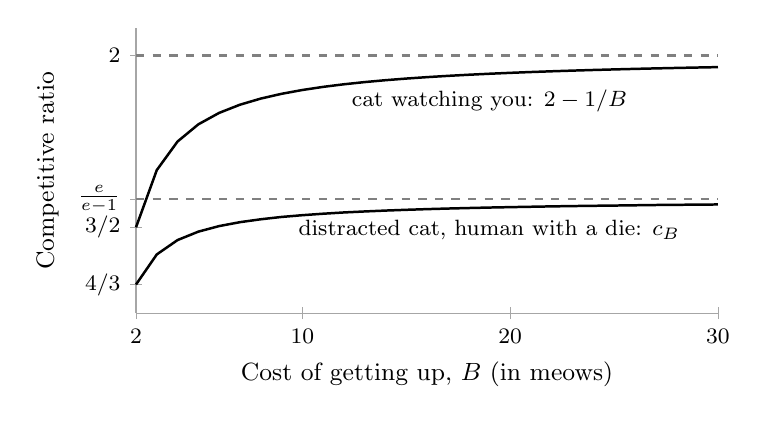
\begin{tikzpicture}
\begin{axis}[
  revista,
  xlabel={Cost of getting up, $B$ (in meows)},
  ylabel={Competitive ratio},
  xmin=2, xmax=30,
  ymin=1.25, ymax=2.08,
  xtick={2,10,20,30},
  ytick={1.333,1.5,1.582,2},
  yticklabels={$4/3$,$3/2$,$\tfrac{e}{e-1}$,$2$}
]
\addplot[gray, dashed] coordinates {(2,2) (30,2)};
\addplot[gray, dashed] coordinates {(2,1.58198) (30,1.58198)};
\addplot[black, samples at={2,3,...,30}] {2-1/x};
\addplot[black, samples at={2,3,...,30}] {1/(1-(1-1/x)^x)};
\node[font=\footnotesize, anchor=north] at (axis cs:19,1.93) {cat watching you: $2-1/B$};
\node[font=\footnotesize, anchor=north] at (axis cs:19,1.55) {distracted cat, human with a die: $c_B$};
\end{axis}
\end{tikzpicture}
\caption{The value of randomness. Rolling a die at 3\,a.m.\ helps only if the cat is not watching.}\label{fig:noche}
\end{figure}

With $B=10$\calib, the best deterministic policy pays $1.9$ times the optimum and the randomized one $1.535$ (Figure~\ref{fig:noche}), with $p_1\approx 0.060$ and $p_{10}\approx 0.154$: the willingness to give in grows geometrically with each meow. The practical recommendation is to roll a die, provided the cat does not see you roll it. The cat is watching you.

\subsection{Where is Miko?}

\begin{definicion}[Searching for the cat]
The human keeps a list of $n$ places. If the cat is at position $i$, finding it costs $i$. After finding it, moving that place forward in the list is free; any other adjacent exchange costs $1$. Given a sequence $\sigma$ of $m$ hiding places, $C_A(\sigma)$ is the total cost of policy $A$. The \emph{move-to-front} (MTF) policy consists of looking first where you last saw it.
\end{definicion}

\begin{teorema}[Sleator--Tarjan~\cite{sleator}]\label{teo:mtf}
For every policy $A$ starting from the same list, even a clairvoyant one, $C_{\mathrm{MTF}}(\sigma)\le 2C_A(\sigma)-m$.
\end{teorema}

\begin{proof}
Let the potential $\Phi$ be the number of inversions between the lists of MTF and $A$: the pairs of places appearing in different order. I consider the search for $x$, at position $k$ for MTF and $i$ for $A$, and let $v$ be the number of places before $x$ in MTF but after $x$ in $A$. The other $k-1-v$ places preceding $x$ in MTF also precede it in $A$, so $k-1-v\le i-1$. Moving $x$ to the front creates $k-1-v$ inversions and destroys $v$. The amortized cost of MTF is then
\begin{equation}
  k+(k-1-v)-v=2(k-v)-1\le 2i-1.
\end{equation}
With $x$ already at the front in MTF, the free forward moves of $x$ in $A$ can only remove inversions, and each paid exchange of $A$ creates at most one. Summing over $\sigma$, with $\Phi_0=0\le\Phi_{\mathrm{final}}$ and $X$ the number of paid exchanges, $C_{\mathrm{MTF}}\le\sum(2i-1)+X\le 2C_A-m$.
\end{proof}

\begin{teorema}[It is always in the last place you look]\label{teo:ultimo}
Against every deterministic policy, a cat that always hides in the last place of the human's current list imposes a cost of $mn$, while some fixed policy costs at most $m(n+1)/2+\binom n2$. The ratio tends to $2-2/(n+1)$ as $m\to\infty$.
\end{teorema}

\begin{proof}
The cost $mn$ is immediate. Averaging over the $n!$ fixed lists, each search costs $(n+1)/2$, so some list costs at most $m(n+1)/2$, and reaching it takes at most $\binom n2$ exchanges.
\end{proof}

The popular saying is a tautology, since one stops looking upon finding. What the theorem adds is that the last place can also be the worst. With $n=6$\calib, the ratio is $1.714$, and by Theorem~\ref{teo:mtf}, looking where you last saw it stays within $2/(n+1)$ of the best that theory allows deterministic humans. The cat knows your list: it has watched you search.

\subsection{Colonies: NP-completeness}

\begin{definicion}[Feline interdiction]
The house is a graph $G=(V,E)$. The human, a creature of habit, repeats fixed routes $R_1,\dots,R_m$, each a simple path in $G$. A cat at $v$ blocks every route passing through $v$. For a colony $S\subseteq V$, let $b(S)=|\{i:R_i\cap S\ne\varnothing\}|$. The problem \prob{Interdiction} asks whether there is $S$ with $|S|\le k$ and $b(S)=m$; \prob{Max-Interdiction} maximizes $b(S)$ subject to $|S|\le k$. Let $L=\sum_i|R_i|$ and $d=\max_i|R_i|$.
\end{definicion}

\begin{proposicion}[One cat is easy]\label{prop:ungato}
For $k=1$, the best vertex is found in time $O(L+|V|)$.
\end{proposicion}

\begin{proof}
It suffices to count, in one pass over the routes, how many contain each vertex.
\end{proof}

\begin{teorema}[A colony is hard]\label{teo:npc}
\prob{Interdiction} is NP-complete. Moreover, unless $\mathrm{P}=\mathrm{NP}$, for every $\epsilon>0$ no polynomial-time algorithm approximates \prob{Max-Interdiction} within a factor $1-1/e+\epsilon$.
\end{teorema}

\begin{proof}
Given $S$, I check $b(S)=m$ in time $O(L)$, so the problem is in NP. I reduce from \prob{Vertex Cover}~\cite{karp}: given $(G,k)$, each edge $\{u,v\}$ becomes the route $(u,v)$. A colony blocks all routes if and only if it touches all edges.

For inapproximability, I take an instance of \prob{Max-$k$-Cover} with sets $A_1,\dots,A_N$ over a universe $U$ whose elements each belong to some set. I take as the house the complete graph on $\{1,\dots,N\}$, an open floor plan, and for each $u\in U$ a route traversing $\{i:u\in A_i\}$ in any order, which is a simple path. Then $b(S)$ is exactly the coverage of $S$, and I apply Feige's threshold~\cite{feige}.
\end{proof}

\begin{teorema}[The greedy colony]\label{teo:voraz}
Placing each cat in turn where it blocks the most new routes takes time $O(k(L+|V|))$ and satisfies
\begin{equation}
  b(S_{\mathrm{greedy}})\ge\Bigl[1-\Bigl(1-\frac1k\Bigr)^{k}\Bigr]\OPT>\Bigl(1-\frac1e\Bigr)\OPT.
\end{equation}
By Theorem~\ref{teo:npc}, no polynomial-time algorithm improves this constant asymptotically, unless $\mathrm{P}=\mathrm{NP}$.
\end{teorema}

\begin{proof}
Let $a_i$ be the number of routes blocked after $i$ cats. The $k$ vertices of the optimum block at least $\OPT-a_i$ routes that are still free, so, by pigeonhole, one of them blocks at least $(\OPT-a_i)/k$. Hence $\OPT-a_{i+1}\le(1-1/k)(\OPT-a_i)$, and I iterate from $a_0=0$~\cite{nemhauser}. Each turn is one counting pass.
\end{proof}

\begin{teorema}[Short routes, few cats]\label{teo:fpt}
\prob{Interdiction} is decidable in time $O(d^{\,k}L)$ for $d\ge 2$. In particular, it is fixed-parameter tractable in $k+d$.
\end{teorema}

\begin{proof}
I take a free route. Every solution must place a cat on one of its at most $d$ vertices, so I branch on them and solve with $k-1$ cats on the remaining routes. If $T(k)$ is the running time, $T(k)\le d\,T(k-1)+O(dL)$ with $T(0)=O(L)$, and this recurrence gives $T(k)=O(d^{\,k}L)$, since the geometric sum is dominated by the last level.
\end{proof}

\begin{table}[ht]
\centering
\caption{Summary of algorithmic results.}\label{tab:algoritmos}
\begin{tabular}{lll}
\toprule
Situation & Problem & Result \\
\midrule
3\,a.m., watching cat & \emph{ski rental} & $2-1/B$, tight \\
3\,a.m., distracted cat & randomized \emph{ski rental} & $c_B\to e/(e-1)$, tight \\
Searching for the cat & \emph{list update} & $\le 2$; $\ge 2-2/(n+1)$ \\
One blocking cat & counting & $O(L+|V|)$ \\
$k$ cats, total blockage & cover & NP-complete \\
$k$ cats, approximate & greedy & $1-1/e$, threshold \\
$k$ cats, short routes & search tree & $O(d^{\,k}L)$ \\
\bottomrule
\end{tabular}
\end{table}

\begin{observacion}[The same constant]
The factor in Theorem~\ref{teo:voraz} with $k=B$ is exactly $1/c_B$: the expression $1-(1-1/x)^x$ governs both what a greedy colony achieves and what a human with a die pays. I claim no duality here; I merely record that the number $e$ has a cat too.
\end{observacion}

\begin{observacion}[On P versus NP]
If $\mathrm{P}=\mathrm{NP}$, I could compute the optimal colony in polynomial time. The harder problem, getting the cats to sit there, remains open.
\end{observacion}

\section{Minor results}\label{sec:menores}

\begin{proposicion}[The glass]\label{prop:vaso}
Pushing an object of mass $m$ a distance $d$ to the edge with friction $\mu_f$ costs $\mu_f mgd$ and releases $mgh$ on falling from height $h$. The energy gain
\begin{equation}
  \mathcal A=\frac{h}{\mu_f d}
\end{equation}
does not depend on $m$.
\end{proposicion}

With $h=75$\,cm, $\mu_f=0.3$ and $d=5$\,cm\calib, the gain is $\mathcal A=50$. Few capital investments return as much, and since the gain is independent of mass, the cat can choose the object solely by the expected volume of the human's scream. That is, surely, the variable being maximized.

\begin{proposicion}[Lapping, Reis et al.~\cite{reis}]\label{prop:lengua}
Let $\mathrm{Fr}^{*}=(R/H)\,\mathrm{Fr}^{2/3}$, with $\mathrm{Fr}=U/\sqrt{gR}$, where $U$ is the maximum tongue speed, $R$ its radius and $H$ the lapping height. If the frequency is tuned so that the mouth closes as the column collapses, $\mathrm{Fr}^{*}$ is of order one, and if the family is isometric, then $f\sim M^{-1/6}$.
\end{proposicion}

This derivation is due to Reis et al., not to me. With their values ($U=78$\,cm/s, $H=3$\,cm, $R\approx 5$\,mm), I get $\mathrm{Fr}^{*}\approx 0.39$. Their fit across eight feline species gives $f=4.6\,M^{-0.181\pm 0.024}$, compatible with $-1/6$; at $4$\,kg it predicts $3.58$\,s$^{-1}$, against the measured $3.5\pm0.4$\,s$^{-1}$. A tiger and an apartment cat obey the same dimensionless number without having consulted it.

\begin{proposicion}[The sphere and the keyboard]\label{prop:esfera}
Among all bodies of volume $V$, the sphere minimizes surface area: $A\ge(36\pi)^{1/3}V^{2/3}$. If heat loss is $hA(T_b-T_a)$ and metabolism is $M$, then with no other sources the cat can only balance in the range $T_a\ge T_b-M/(hA_{\text{sphere}})$. Below it, the deficit of a sphere is $hA_{\text{sphere}}(T_b-T_a)-M>0$.
\end{proposicion}

A $4$\,kg cat with the density of water\calib\ has a sphere of radius $9.85$\,cm and $A=0.122$\,m$^2$, against $0.168$\,m$^2$ for a stretched $45$\,cm cylinder\calib: curling up saves $27.5\%$ of the surface. The veterinary formula $70\,M^{0.75}$ gives $M\approx 9.6$\,W. I calibrate $h\approx 9.3$\,W\,m$^{-2}$K$^{-1}$ by matching the lower edge to the $30\,^\circ$C of the reported thermoneutral zone of $30$ to $38\,^\circ$C~\cite{nrc}, with $T_b=38.5\,^\circ$C\calib.

The model then predicts that the cat moves from sphere to cylinder between $30$ and $32.3\,^\circ$C. More importantly, in a room at $20\,^\circ$C, the curled cat runs a deficit of $11.3$\,W, right around the order of magnitude a laptop dissipates. Sitting on your keyboard is therefore not sabotage but the solution of a heat balance that also, as a free side effect, captures all of your attention. The point is Pareto-optimal, and your productivity is not among its objectives.

\section{Open problems}\label{sec:abiertos}

\begin{conjetura}[Nocturnal garbage collection]
Every domestic cat traverses the house at top speed during some interval near 3\,a.m., and this process serves as garbage collection over an unobservable internal state. I know of no proof, although much human sleep has been sacrificed in the attempt.
\end{conjetura}

\begin{problema}[Gift versus box]
Let $G$ be a gift of arbitrary price and $B$ the box it came in. Prove that $u(B)>u(G)$ for all $G$, or construct a counterexample. Vinke et al.~\cite{vinke} and Smith et al.~\cite{smith} suggest that the effect persists even in the limiting case where $B$ is drawn on the floor.
\end{problema}

\begin{problema}[Gittins index of the glass]
Compute the Gittins index of each object on the table as an arm of a bandit whose reward is the human's reaction. The optimal policy, known experimentally, starts with the most expensive one.
\end{problema}

\begin{problema}[The non-abelian case]
Extend the bounds of \S\ref{sec:caida} to the Kane--Scher model, with group $SO(3)$. This looks feasible. Getting the cat to cooperate with experimental validation does not.
\end{problema}

\section{Conclusion}

I have shown that a set of behaviors considered capricious (the staring, the meow after dinner, the 3\,a.m.\ concert, the uncrossed door, the move into the sun, the glass on the floor, the occupied keyboard) admits a description as solutions to well-posed optimization problems, and in several cases attains exact bounds. The title of expert is not rhetorical: the cat operates on the frontier of the possible, under incomplete information, and without having read any of this.

The natural question is whether the cat knows what it is doing. By the preceding theorems the question is irrelevant to the outcome, and, by Proposition~\ref{prop:noComputable}, possibly impossible to answer. I leave it to the reader to decide how comfortable to feel about that, preferably while opening a door for someone.

\bigskip
\noindent\textbf{Declarations.} \emph{Data and code:} my program \texttt{revision\_por\_patas.py} reproduces every number in this work; it lives, together with the source, at \href{https://github.com/stiffis/complejidad-gatuna}{\nolinkurl{github.com/stiffis/complejidad-gatuna}}. \emph{Ethics:} I dropped no cat for this study, Miko included; nor did I ask for consent, since I already knew the outcome. \emph{Competing interests:} I am, in the sense of Definition~\ref{def:sistema}, a human, and specifically Miko's human.

\medskip
\noindent\textbf{Acknowledgments.} I thank Miko, my cat, for inspiring this work. Miko has not read the manuscript, and I do not expect that to change.

\begin{thebibliography}{99}
\small
\bibitem{banchoffpohl} T.~Banchoff and W.~F.~Pohl. A generalization of the isoperimetric inequality. \emph{J.\ Differential Geometry} 6 (1971), 175--192.
\bibitem{bendavid} S.~Ben-David, A.~Borodin, R.~Karp, G.~Tardos and A.~Wigderson. On the power of randomization in on-line algorithms. \emph{Algorithmica} 11 (1994), 2--14.
\bibitem{charnov} E.~L.~Charnov. Optimal foraging, the marginal value theorem. \emph{Theoretical Population Biology} 9(2) (1976), 129--136.
\bibitem{delgado} M.~M.~Delgado, B.~S.~G.~Han and M.~J.~Bain. Domestic cats (\emph{Felis catus}) prefer freely available food over food that requires effort. \emph{Animal Cognition} (2021). doi:10.1007/s10071-021-01530-3.
\bibitem{dixitpindyck} A.~K.~Dixit and R.~S.~Pindyck. \emph{Investment under Uncertainty}. Princeton University Press, 1994.
\bibitem{fardin} M.-A.~Fardin. On the rheology of cats. \emph{Rheology Bulletin} 83(2) (2014), 16--17 and 30.
\bibitem{feige} U.~Feige. A threshold of $\ln n$ for approximating set cover. \emph{Journal of the ACM} 45(4) (1998), 634--652.
\bibitem{kamenica} E.~Kamenica and M.~Gentzkow. Bayesian persuasion. \emph{American Economic Review} 101(6) (2011), 2590--2615.
\bibitem{kanescher} T.~R.~Kane and M.~P.~Scher. A dynamical explanation of the falling cat phenomenon. \emph{International Journal of Solids and Structures} 5 (1969), 663--670.
\bibitem{karlin} A.~R.~Karlin, M.~S.~Manasse, L.~A.~McGeoch and S.~Owicki. Competitive randomized algorithms for nonuniform problems. \emph{Algorithmica} 11(6) (1994), 542--571.
\bibitem{karp} R.~M.~Karp. Reducibility among combinatorial problems. In R.~E.~Miller and J.~W.~Thatcher (eds.), \emph{Complexity of Computer Computations}. Plenum Press (1972), 85--103.
\bibitem{kolmogorov} A.~N.~Kolmogorov. Three approaches to the quantitative definition of information. \emph{Problems of Information Transmission} 1(1) (1965), 1--7.
\bibitem{livitanyi} M.~Li and P.~Vitányi. \emph{An Introduction to Kolmogorov Complexity and Its Applications}. Springer.
\bibitem{marey} É.-J.~Marey. Des mouvements que certains animaux exécutent pour retomber sur leurs pieds, lorsqu'ils sont précipités d'un lieu élevé. \emph{Comptes Rendus de l'Académie des Sciences} 119 (1894), 714--717.
\bibitem{marey-nature} Photographs of a tumbling cat. \emph{Nature} 51 (1894), 80--81.
\bibitem{mccomb} K.~McComb, A.~M.~Taylor, C.~Wilson and B.~D.~Charlton. The cry embedded within the purr. \emph{Current Biology} 19(13) (2009), R507--R508.
\bibitem{mcdonaldsiegel} R.~McDonald and D.~Siegel. The value of waiting to invest. \emph{Quarterly Journal of Economics} 101(4) (1986), 707--727.
\bibitem{montgomery} R.~Montgomery. Gauge theory of the falling cat. In M.~J.~Enos (ed.), \emph{Dynamics and Control of Mechanical Systems: The Falling Cat and Related Problems}. Fields Institute Communications 1, AMS (1993), 193--218.
\bibitem{moore} I.~Moore. \emph{Six-Dinner Sid}. 1990. Picture book; case study with $n=6$.
\bibitem{nemhauser} G.~L.~Nemhauser, L.~A.~Wolsey and M.~L.~Fisher. An analysis of approximations for maximizing submodular set functions, I. \emph{Mathematical Programming} 14 (1978), 265--294.
\bibitem{nrc} National Research Council. \emph{Nutrient Requirements of Dogs and Cats}. National Academies Press, 2006.
\bibitem{reis} P.~M.~Reis, S.~Jung, J.~M.~Aristoff and R.~Stocker. How cats lap: water uptake by \emph{Felis catus}. \emph{Science} 330 (2010), 1231--1234. doi:10.1126/science.1195421.
\bibitem{saito} A.~Saito, K.~Shinozuka, Y.~Ito and T.~Hasegawa. Domestic cats (\emph{Felis catus}) discriminate their names from other words. \emph{Scientific Reports} 9 (2019), 5394. doi:10.1038/s41598-019-40616-4.
\bibitem{shannon} C.~E.~Shannon. A mathematical theory of communication. \emph{Bell System Technical Journal} 27 (1948), 379--423 and 623--656.
\bibitem{sleator} D.~D.~Sleator and R.~E.~Tarjan. Amortized efficiency of list update and paging rules. \emph{Communications of the ACM} 28(2) (1985), 202--208.
\bibitem{smith} G.~E.~Smith, P.~A.~Chouinard and S.-E.~Byosiere. If I fits I sits: a citizen science investigation into illusory contour susceptibility in domestic cats (\emph{Felis silvestris catus}). \emph{Applied Animal Behaviour Science} 240 (2021), 105338.
\bibitem{vinke} C.~M.~Vinke, L.~M.~Godijn and W.~J.~R.~van der Leij. Will a hiding box provide stress reduction for shelter cats? \emph{Applied Animal Behaviour Science} 160 (2014), 86--93.
\bibitem{yao} A.~C.-C.~Yao. Probabilistic computations: toward a unified measure of complexity. \emph{Proc.\ 18th IEEE Symposium on Foundations of Computer Science} (1977), 222--227.
\end{thebibliography}

\end{document}
